\begin{pastexam}[label={px:ntu-109-dsaa-04}]{臺大資工所 109 學年度 第 4 題}
（複選；正確的選項可能有 0 到 5 個，都不對時答 none）

(3 points) A \textit{binary minimum heap} is a binary tree in which every level is completely
full, except the last level, which is filled from the left to right. Here the \textit{level} of a
node is its distance to the root, so the root has level 0 and the children of the root will have
level 1, and so on. Also the key of a parent is less than those of its children. For ease of
discussion we assume that all keys in the heap are \textit{distinct}. Now which of the following
descriptions about a binary minimum heap of \textit{10} nodes (see the figure below) are correct?

\begin{center}
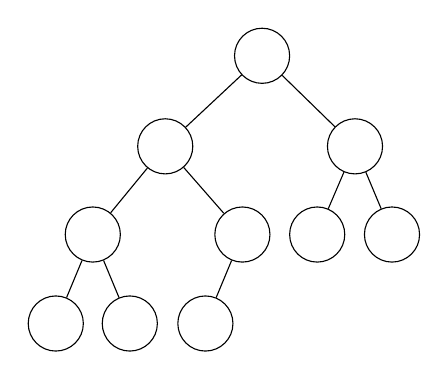
\begin{tikzpicture}[n/.style={circle,draw,inner sep=0pt,minimum size=7mm}]
\node[n] (a) at (0.00,0.00) {};
\node[n] (b) at (-1.23,-1.15) {};
\node[n] (c) at (1.18,-1.15) {};
\node[n] (d) at (-2.15,-2.27) {};
\node[n] (e) at (-0.25,-2.27) {};
\node[n] (f) at (0.70,-2.27) {};
\node[n] (g) at (1.65,-2.27) {};
\node[n] (h) at (-2.62,-3.40) {};
\node[n] (i) at (-1.68,-3.40) {};
\node[n] (j) at (-0.72,-3.40) {};
\draw (a)--(b) (a)--(c) (b)--(d) (b)--(e) (c)--(f) (c)--(g) (d)--(h) (d)--(i) (e)--(j);
\end{tikzpicture}
\end{center}

\begin{enumerate}[label=\arabic*.]
\item The second smallest key is always in level 1.
\item The largest key is always in a leaf, i.e., a node without any children.
\item The second largest key is always in a leaf.
\item Let $n$ be the number of nodes and we consider the case of arbitrary $n$, then the height
of the tree is $\Theta(\log n)$.
\item Let $n$ be the number of nodes and we consider the case of arbitrary $n$, then we can find
the \textit{third} smallest key of the heap by $O(1)$ key comparisons.
\end{enumerate}
\end{pastexam}

\begin{pastsoln}
答案：1、2、4、5。

下面用陣列的位置 $1..10$ 稱呼節點（位置 $i$ 的子節點是 $2i$、$2i + 1$，資結書第~8.1.1~節）；圖中位置
$5$ 只有一個子節點（位置 $10$），位置 $6..10$ 是葉節點。 整個推理只用一件事：堆積性質讓每一條從根往下
的路徑都是遞增的，所以\textbf{一個鍵的所有祖先都比它小}。 一個鍵如果是第 $k$ 小，它比它小的只有
$k - 1$ 個，所以它的祖先最多 $k - 1$ 個，深度（level）$\le k - 1$。

\begin{itemize}
\item 1. 第二小的鍵：它的祖先都比它小，比它小的只有最小值，而最小值在根。 所以它的祖先只有根，它是根的
子節點，在 level 1。 對。
\item 2. 最大的鍵：如果它有子節點，子節點的鍵要比它大，不可能。 所以它一定在葉節點。 對。
\item 3. 第二大的鍵：它可以有一個子節點，就是最大的鍵。 反例：陣列
\[
\langle 1, 2, 3, 4, 9, 5, 6, 7, 8, 10\rangle .
\] 檢查堆積性質：位置 $2$ 的 $2$ 小於子節點 $4$、$9$；位置 $3$ 的 $3$ 小於 $5$、$6$；位置
$4$ 的 $4$ 小於 $7$、$8$；位置 $5$ 的 $9$ 小於它唯一的子節點 $10$。 第二大的 $9$ 在位置 $5$，不是
葉節點。 錯。
\item 4. 有 $n$ 個節點的完整二元樹，最深的節點在 level $\lfloor \lg n \rfloor$；資結書定理~7.3 用節點數算
高度，是 $\lfloor \lg n \rfloor + 1$。 不管用哪一種算法，高度都是 $\Theta(\log n)$。 對。 $n = 10$ 時
最深的 level 是 $3$，和圖一樣。
\item 5. 第三小的鍵：由上面的推理它的深度 $\le 2$。 更精確地說，它的祖先是比它小的兩個鍵的一部分，
所以它不是根的子節點，就是「第二小那個節點」的子節點。 做法：
\begin{enumerate}[label=(\roman*)]
\item 比較根的兩個子節點，較小的是第二小，記作 $x$；另一個記作 $y$。 （$1$ 次）
\item 第三小是 $y$ 和 $x$ 的子節點（最多兩個）之中最小的。 （最多 $2$ 次）
\end{enumerate}
最多 $3$ 次比較，和 $n$ 無關，是 $O(1)$。 對。 （$n < 3$ 時沒有第三小，題目考慮的是一般的 $n$。）
\end{itemize}
\end{pastsoln}
